\documentclass[a4paper]{article}
\usepackage[german]{babel}
%\usepackage{libertine}
%\renewcommand*\familydefault{\sfdefault}  %%
\usepackage[default]{opensans}
%\usepackage{gillius2}
%\usepackage{lato}
\usepackage[version=4]{mhchem}

\usepackage[utf8]{inputenc}

\usepackage[T1]{fontenc}

%\usepackage[activate={true,nocompatibility},final,tracking=true,kerning=true,spacing=true,factor=1100,stretch=10,shrink=10]{microtype}

\usepackage[utf8]{inputenc}
\usepackage[T1]{fontenc}

\usepackage{libertine}
\usepackage{microtype}

\usepackage{xcolor,multido}
\usepackage{tikz}
\usepackage{pgffor}
\usepackage{graphicx}
\usepackage[left=1cm,right=1cm,top=1.5cm,bottom=2cm]{geometry}



\begin{document}
\begin{tikzpicture}
\node[inner sep=0pt] (fg0) at (0,0)
    {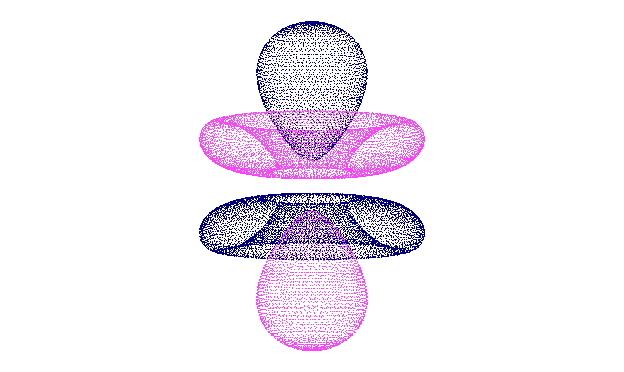
\includegraphics[width=\textwidth]{fg0.png}};
    % The axes
\draw[->,ultra thick] (xyz cs:x=-6.5) -- (xyz cs:x=8) node[above] {\Huge x};
\draw[->,ultra thick] (xyz cs:y=-6.5) -- (xyz cs:y=8) node[right] {\Huge z};
\draw[->,ultra thick] (xyz cs:z=-6.5) -- (xyz cs:z=8) node[above] {\Huge y};

\end{tikzpicture}

\begin{tikzpicture}
\node[inner sep=0pt] (fg1) at (0,0)
    {
\includegraphics[width=\textwidth]{pics/fig0.png}};
    % The axes
\draw[->,ultra thick] (xyz cs:x=0.5) -- (xyz cs:x=6.5) node[above] {\Large x};
\draw[->,ultra thick] (xyz cs:y=0.5) -- (xyz cs:y=6.5) node[right] {\Large y};
\draw[->,ultra thick] (xyz cs:z=0.5) -- (xyz cs:z=6.5) node[above] {\Large z};

\end{tikzpicture}


\begin{tikzpicture}[scale=1.2]
\node[inner sep=0pt] (fg2) at (0,0)
    {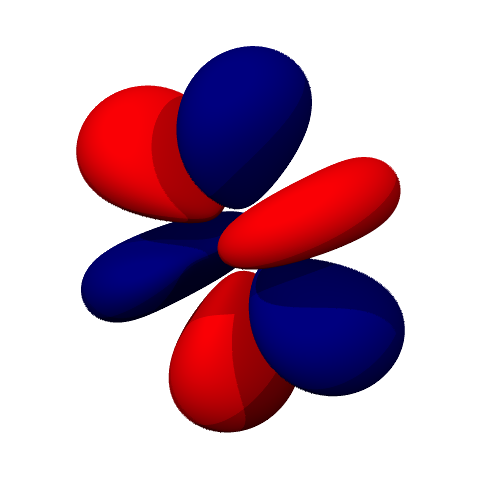
\includegraphics{pics/fig1n.png}};
    % The axes
\draw[->,ultra thick] (xyz cs:x=0.5) -- (xyz cs:x=6.5) node[above] {\Large x};
\draw[->,ultra thick] (xyz cs:y=-0.5) -- (xyz cs:y=6.5) node[right] {\Large y};
\draw[->,ultra thick] (xyz cs:z=-0.5) -- (xyz cs:z=6.5) node[above] {\Large z};
\end{tikzpicture}


\begin{tikzpicture}[scale=1.2]
\node[inner sep=0pt] (fg2) at (0,0)
    {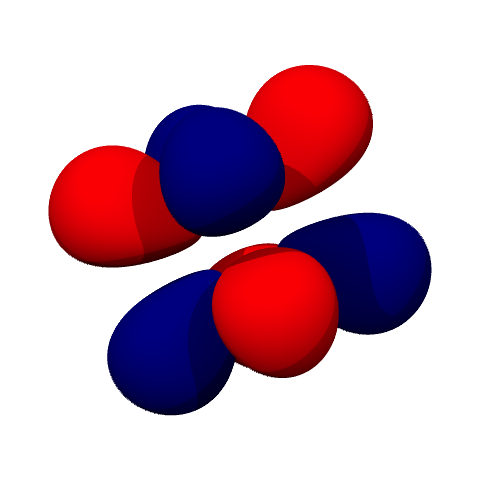
\includegraphics{pics/fig2n.png}};
    % The axes
\draw[->,ultra thick] (xyz cs:x=0.5) -- (xyz cs:x=6.5) node[above] {\Large x};
\draw[->,ultra thick] (xyz cs:y=0.5) -- (xyz cs:y=6.5) node[right] {\Large y};
\draw[->,ultra thick] (xyz cs:z=0.5) -- (xyz cs:z=6.5) node[above] {\Large z};

\end{tikzpicture}

%\draw (0.2,0) circle (2mm); & \fill[red] (0,0) circle (3mm); \\};

%\draw (0.4,0) circle (2mm); & \fill[red] (0,4) circle (3mm); \\
%\draw [very thick,->] (0,0) |- (my matrix.west);

\end{document}